%
% About the Authors
%

\section*{About the authors}

%
% Peter Rohde
%

\begin{center}
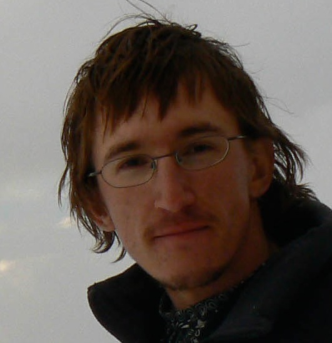
\includegraphics[clip=true, width=0.475\textwidth]{photo_peter_rohde}
\end{center}

\dropcap{P}{eter Rohde} is an Australian Research Council Future Fellow in the Centre for Quantum Software \& Information at the University of Technology Sydney, Australia (UTS:Q$|$SI$\rangle$), and associate member of the Hearne Institute for Theoretical Physics at Louisiana State University. He obtained a Bachelor of Computer Systems Engineering with First Class Honours, and a PhD in theoretical physics at the University of Queensland. He has worked at highly-acclaimed international institutes, including the University of Oxford, University of Queensland, Institute for Molecular Biosciences and Max-Planck Institute for the Science of Light, with over 60 publications and 1,500+ citations in quantum optics, quantum computing, quantum information theory, ecology, and politics. His theoretical proposals have inspired several world-leading experimental efforts, including time-bin encoded \textsc{BosonSampling} and sub-shot-noise limited quantum metrology. He is a collaborator in China's world-first quantum satellite program, aiding in the design of quantum protocols for space-based demonstration. xIn his spare time he is a musician, composer, public speaker, libertarian political activist, charity worker, mountaineer, and adrenaline junkie. He regularly speaks at prominent political and scientific outreach events, features in newspaper and magazine articles, and conducts radio and podcast interviews. He is a very naughty boy and was expelled from preschool\index{Montessori}.

%
% Zixin Huang
%

\begin{center}
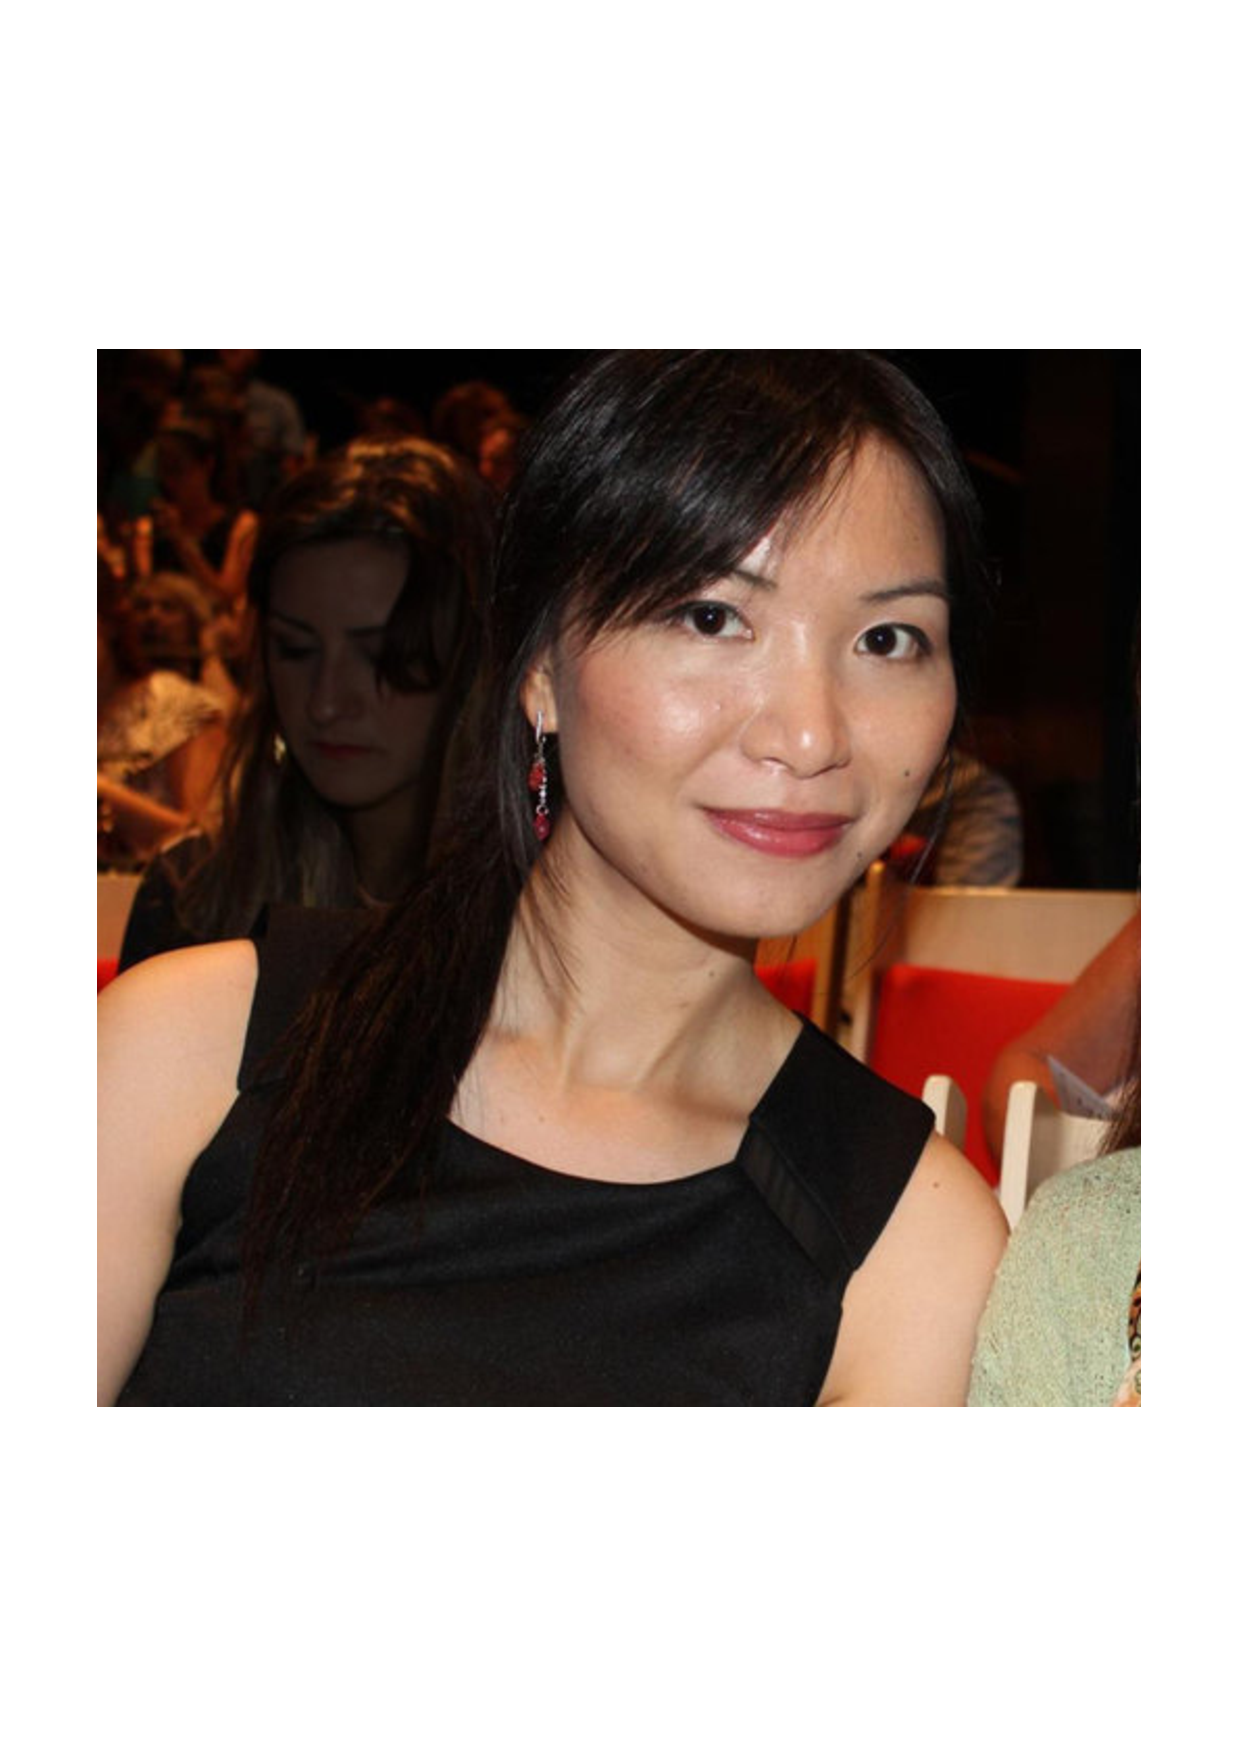
\includegraphics[clip=true, width=0.475\textwidth]{photo_zixin_huang}
\end{center}

\dropcap{Z}{ixin Huang} completed her PhD in physics at the University of Sydney, Australia. She is currently a postdoctoral researcher at the University of Sheffield, UK. She has worked on a wide range of topics ranging from quantum metrology and cryptography to experimental quantum optics. 

% \comment{Complete this section}

%
% He-Liang Huang
%

\begin{center}
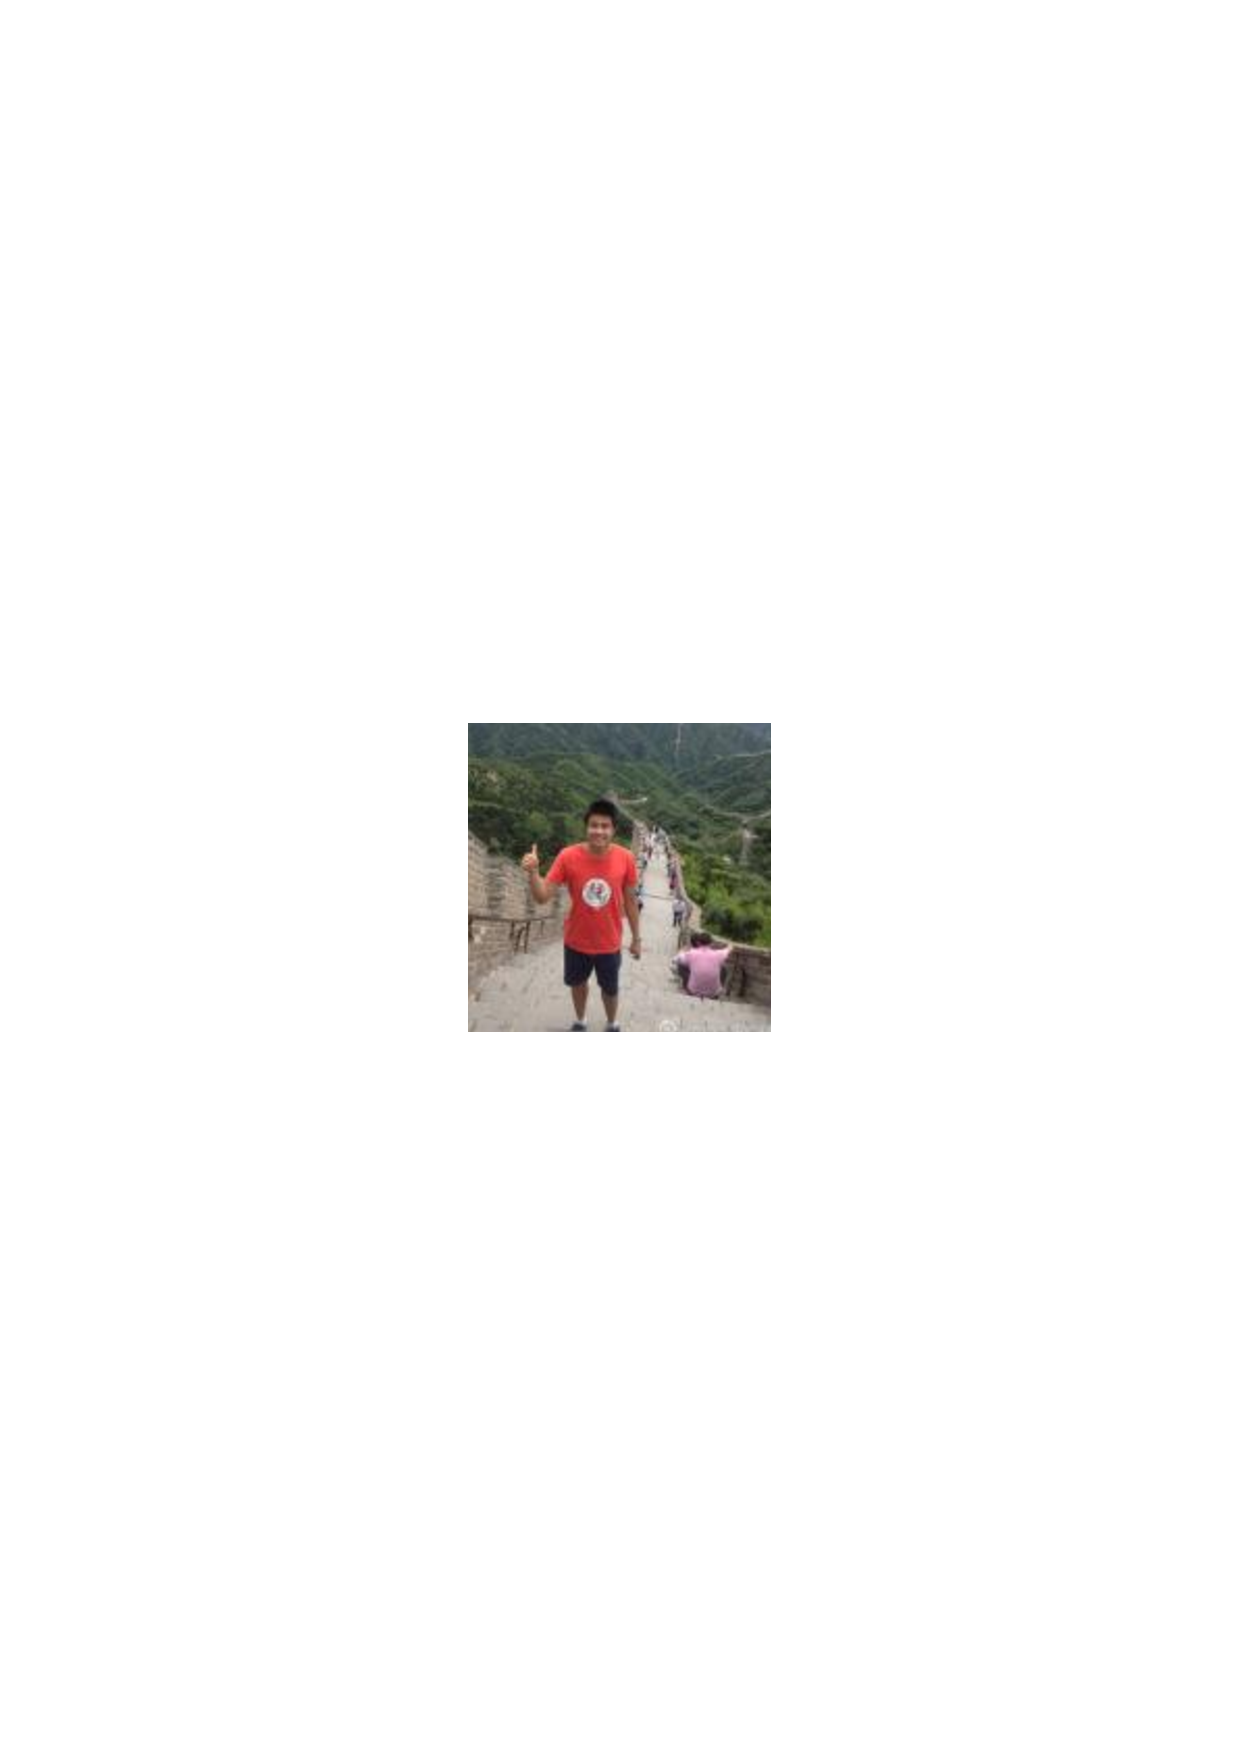
\includegraphics[clip=true, width=0.475\textwidth]{photo_heliang_huang}
\end{center}

\dropcap{H}{e-Liang Huang} is a Postdoctoral Fellow at the University of Science \& Technology China (USTC). His research interests include secure cloud quantum computing, quantum big data analysis, and the physical implementation of quantum computing architectures, in particular using linear optical and superconducting systems. As an experimentalist he has been a part of several groundbreaking experimental efforts, most notably in the demonstration of world-leading multi-photon optical quantum information processing protocols. This includes the first experimental demonstration of topological data analysis on a photonic quantum computer, an optical demonstration of blind quantum computing, and a loophole-free Wheeler-delayed-choice experiment.

%
% Zu-En Su
%

\begin{center}

\includegraphics[clip=true, width=0.475\textwidth]{photo_zuen_su}
\end{center}

\dropcap{Z}{u-En Su} is a Postdoctoral Fellow at the Technion -- Israel Institute of Technology. He obtained his PhD at the University of Science \& Technology China. His research interests currently include the physical implementation of quantum computation and quantum metrology, primarily based on linear optics and solid-state quantum photonics systems.

%
% Simon Devitt
%

\begin{center}
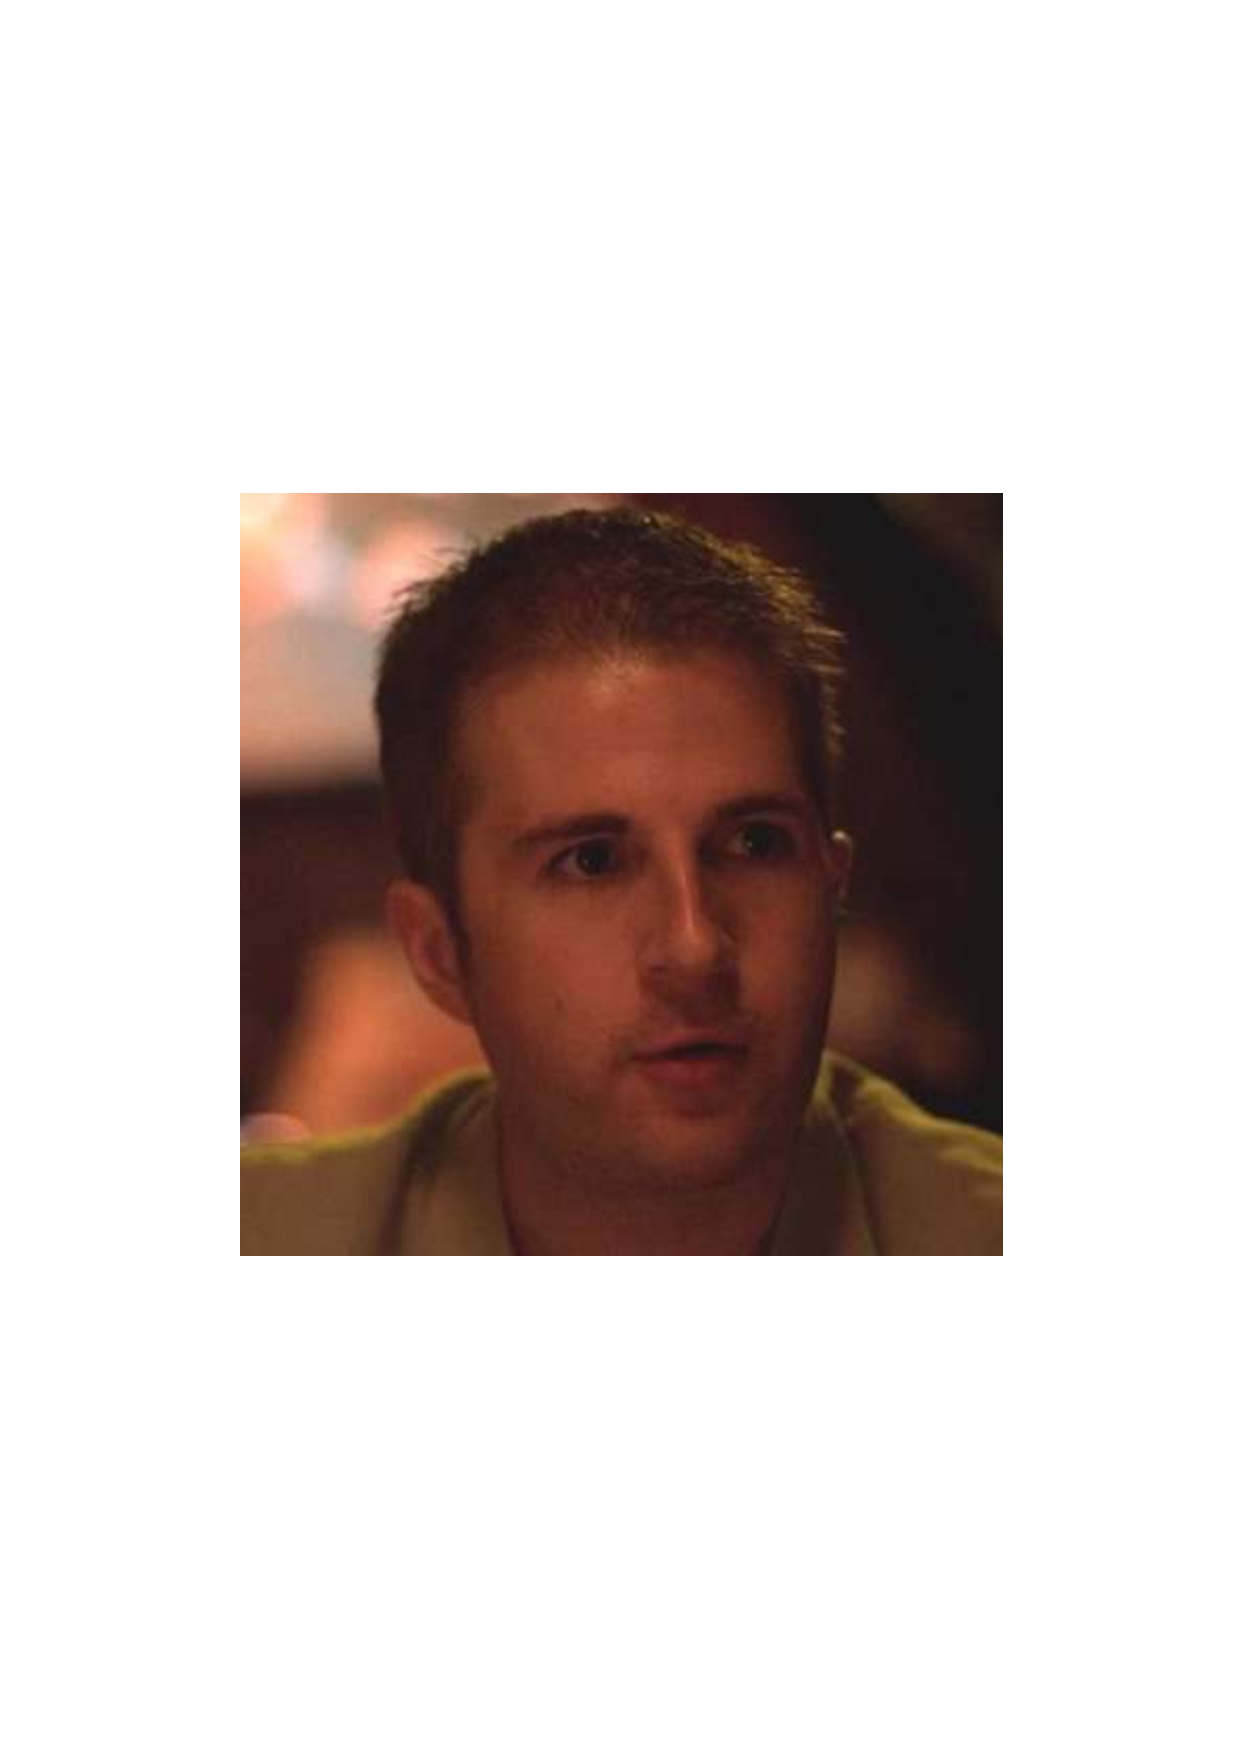
\includegraphics[clip=true, width=0.475\textwidth]{photo_simon_devitt}
\end{center}

\comment{Complete}

\dropcap{S}{imon Devitt}

%
% Rohit Ramakrishnan
%

\begin{center}
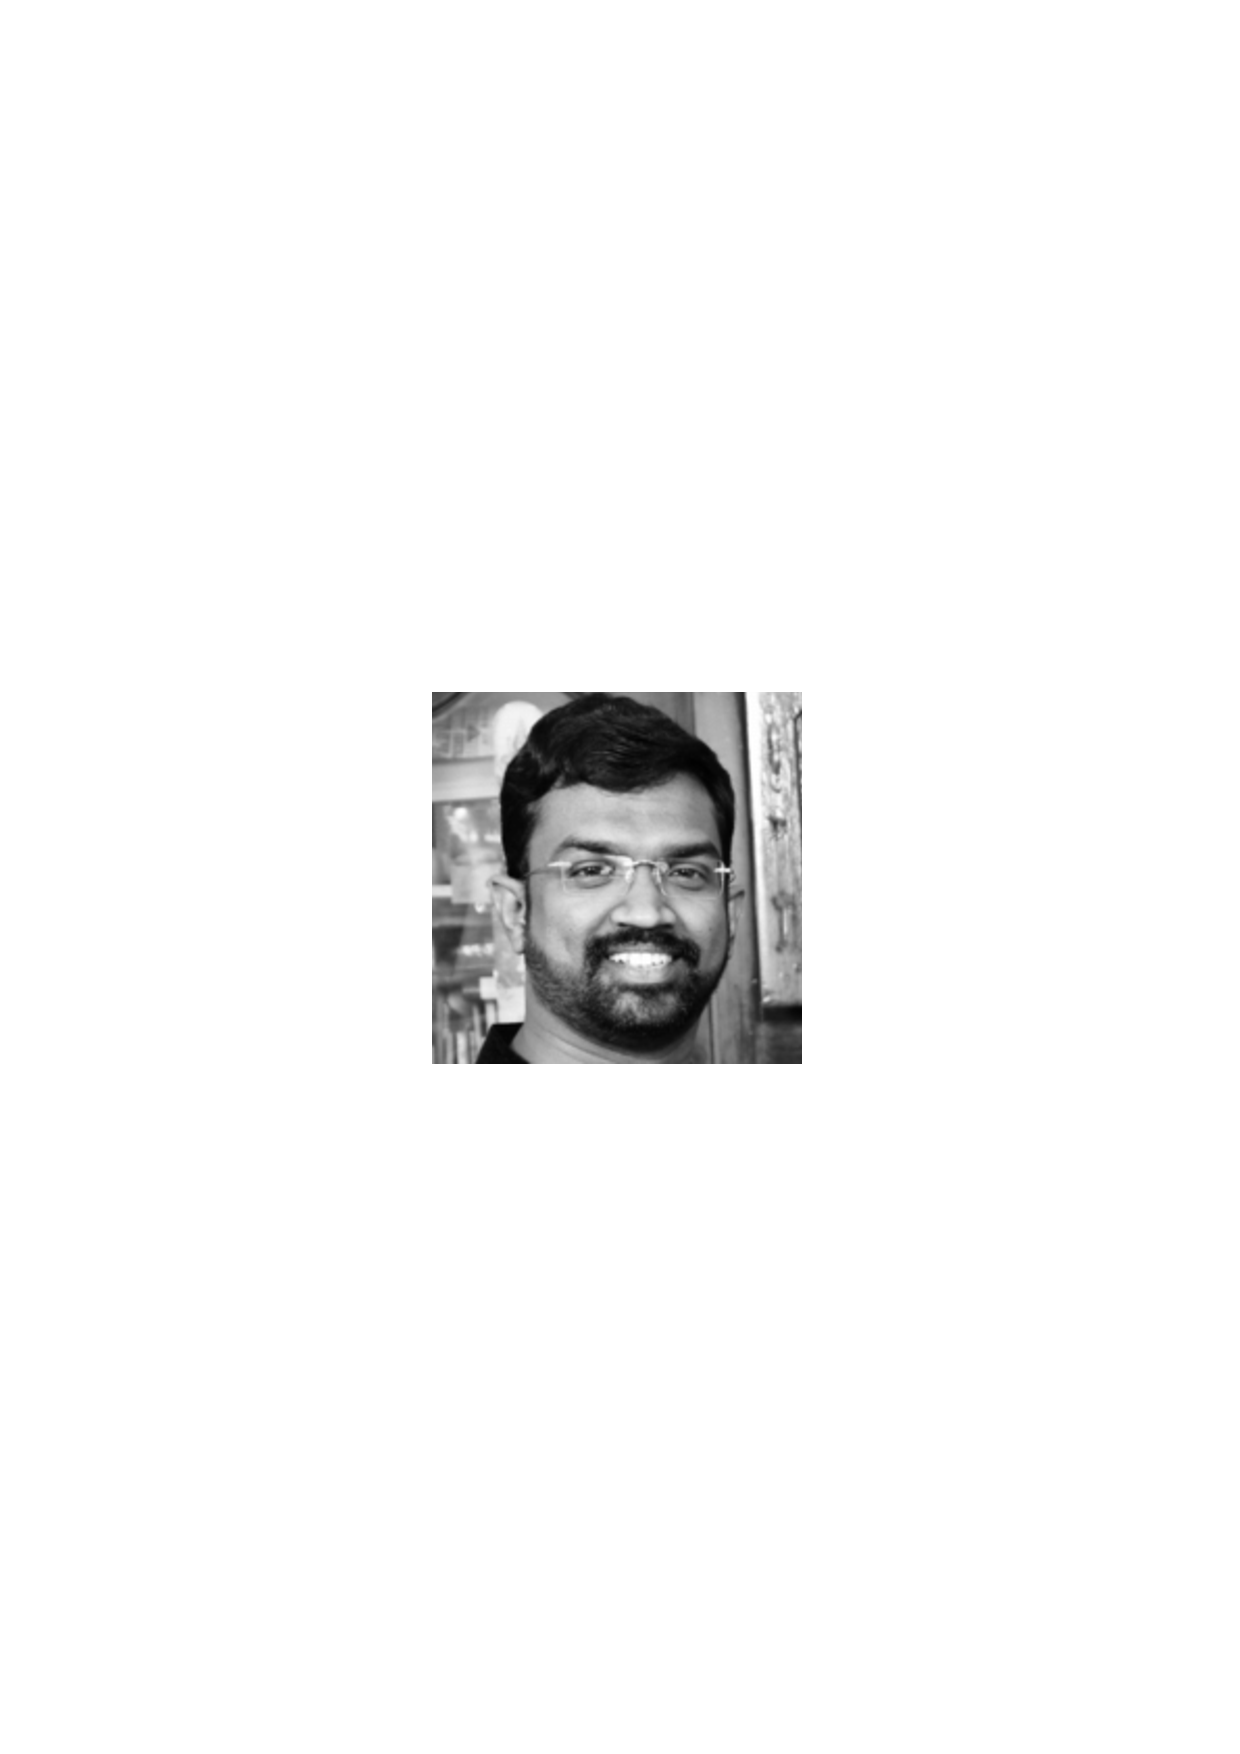
\includegraphics[clip=true, width=0.475\textwidth]{photo_rohit_ramakrishnan}
\end{center}

\dropcap{R}{ohit Ramakrishnan} is a researcher at the Indian Institute of Science.

\comment{Complete this section}

%
% Atul Mantri
%

\begin{center}
%\includegraphics[clip=true, width=0.475\textwidth]{photo_atul_mantri}
\end{center}

\dropcap{A}{tul Mantri} is .... \comment{Complete this section}

%
% Si-Hui Tan
%

\begin{center}
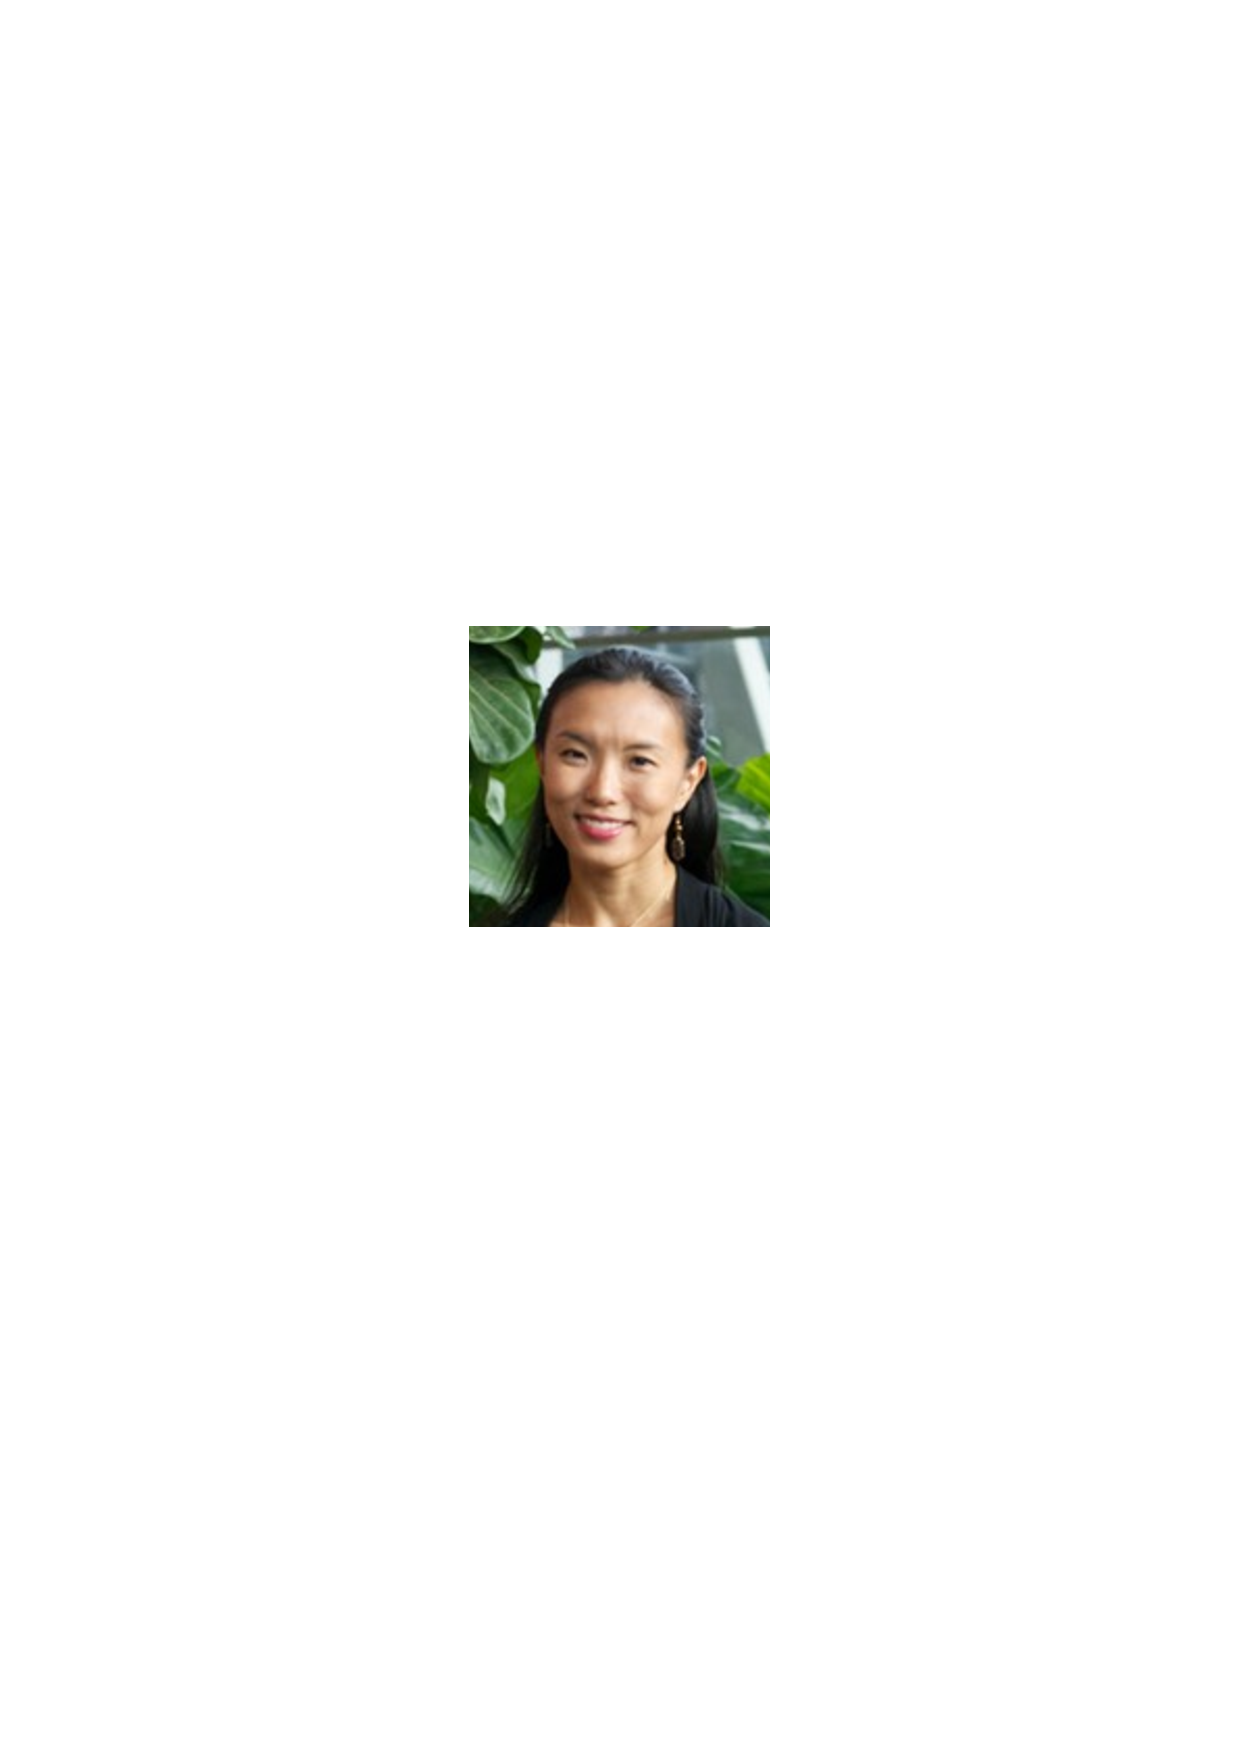
\includegraphics[clip=true, width=0.475\textwidth]{photo_sihui_tan}
\end{center}

\dropcap{S}{i-Hui Tan} is a Research Scientist at the Singapore University of Technology \& Design. She obtained a Bachelor of Science with Honours from Caltech, and subsequently a PhD from MIT. She has received numerous awards, including the MIT Presidential Fellowship.

\comment{Complete this section}

%
% Nana Liu
%

\begin{center}
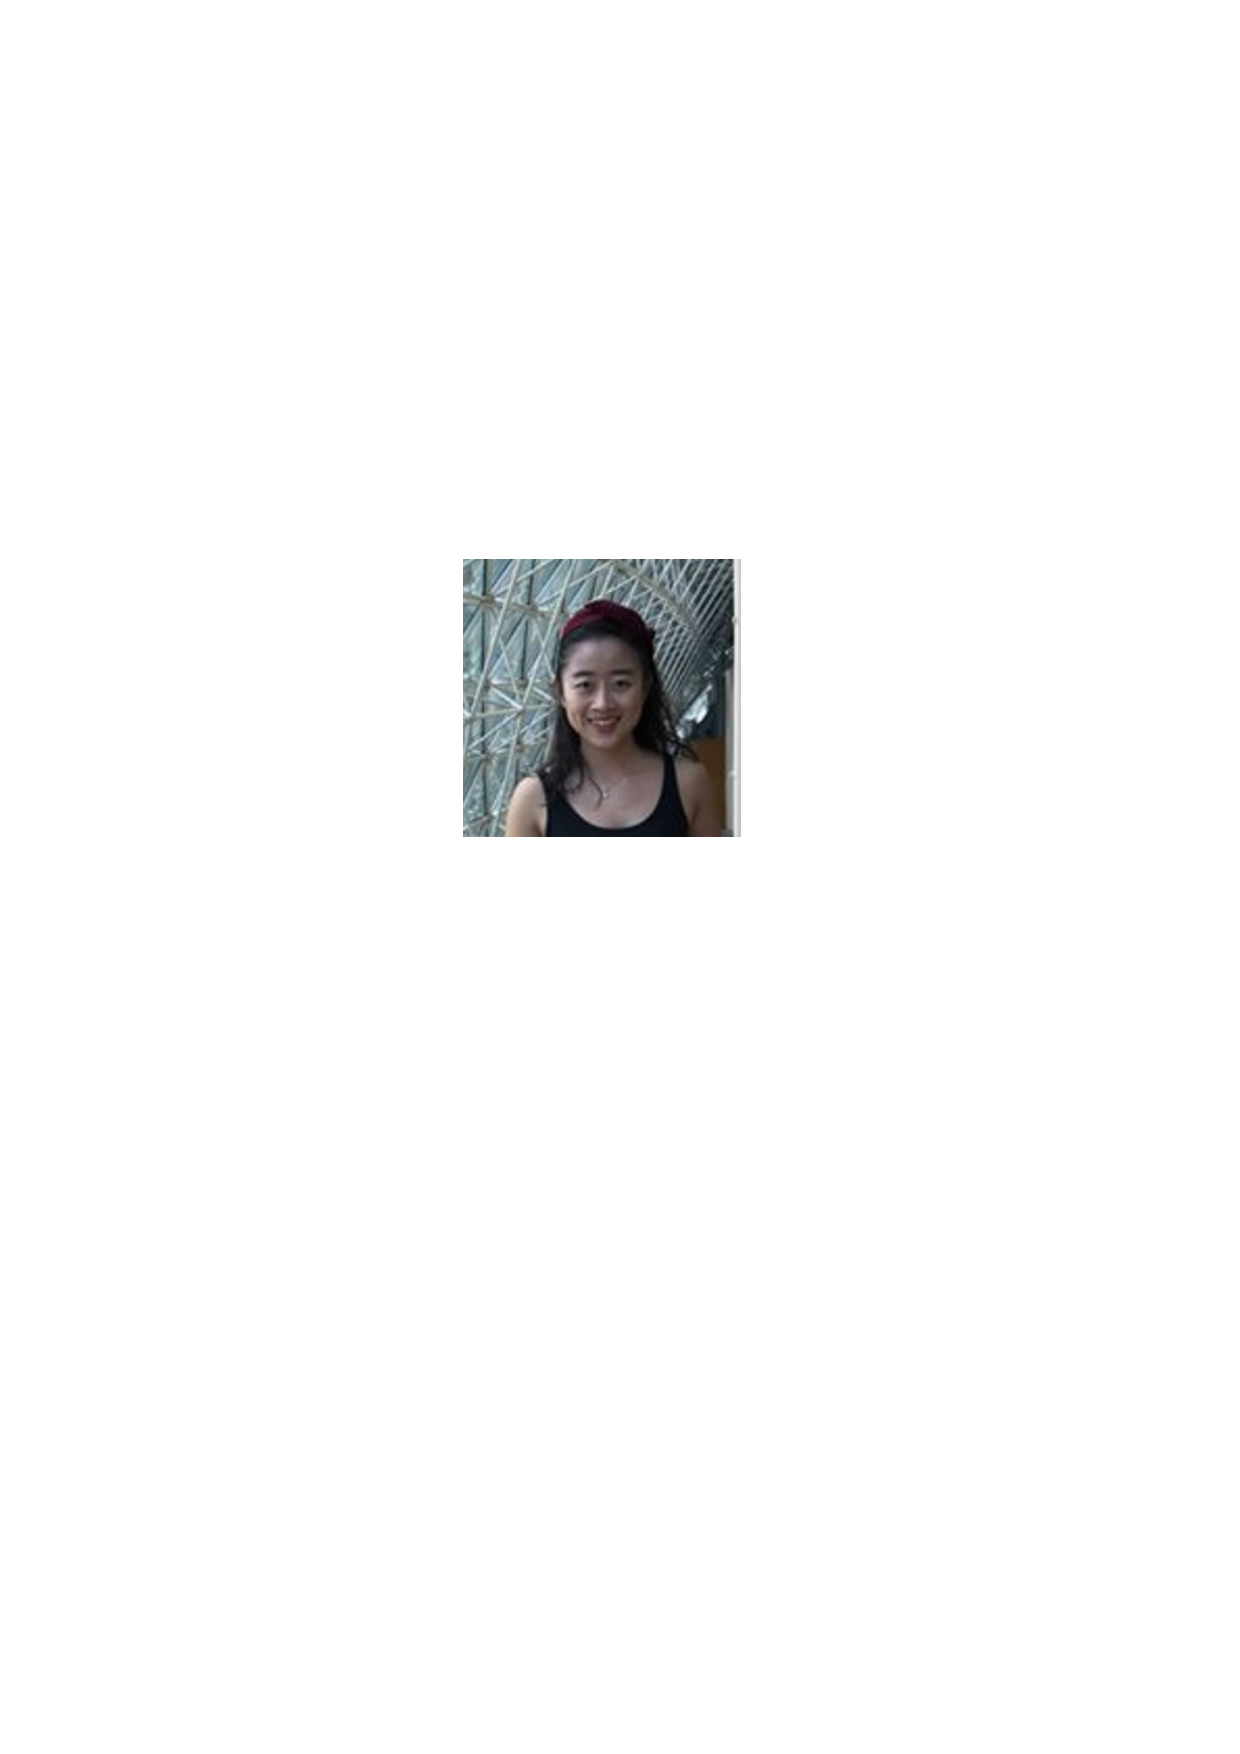
\includegraphics[clip=true, width=0.475\textwidth]{photo_nana_liu}
\end{center}

\dropcap{N}{ana Liu} is a Postdoctoral Research Fellow at the Singapore University of Technology \& Design.

\comment{Complete this section}

%
% Scott Harrison
%

\begin{center}
%\includegraphics[clip=true, width=0.475\textwidth]{photo_scott_harrison}
\end{center}

\dropcap{S}{cott Harrison} is ....\comment{Complete this section}

%
% Darryl Veitch
%

\begin{center}
%\includegraphics[clip=true, width=0.475\textwidth]{photo_darryl_veitch}
\end{center}

\dropcap{D}{arryl Veitch} is .....\comment{Complete this section}

%
% Chandra Radhakrishnan 
%

\begin{center}
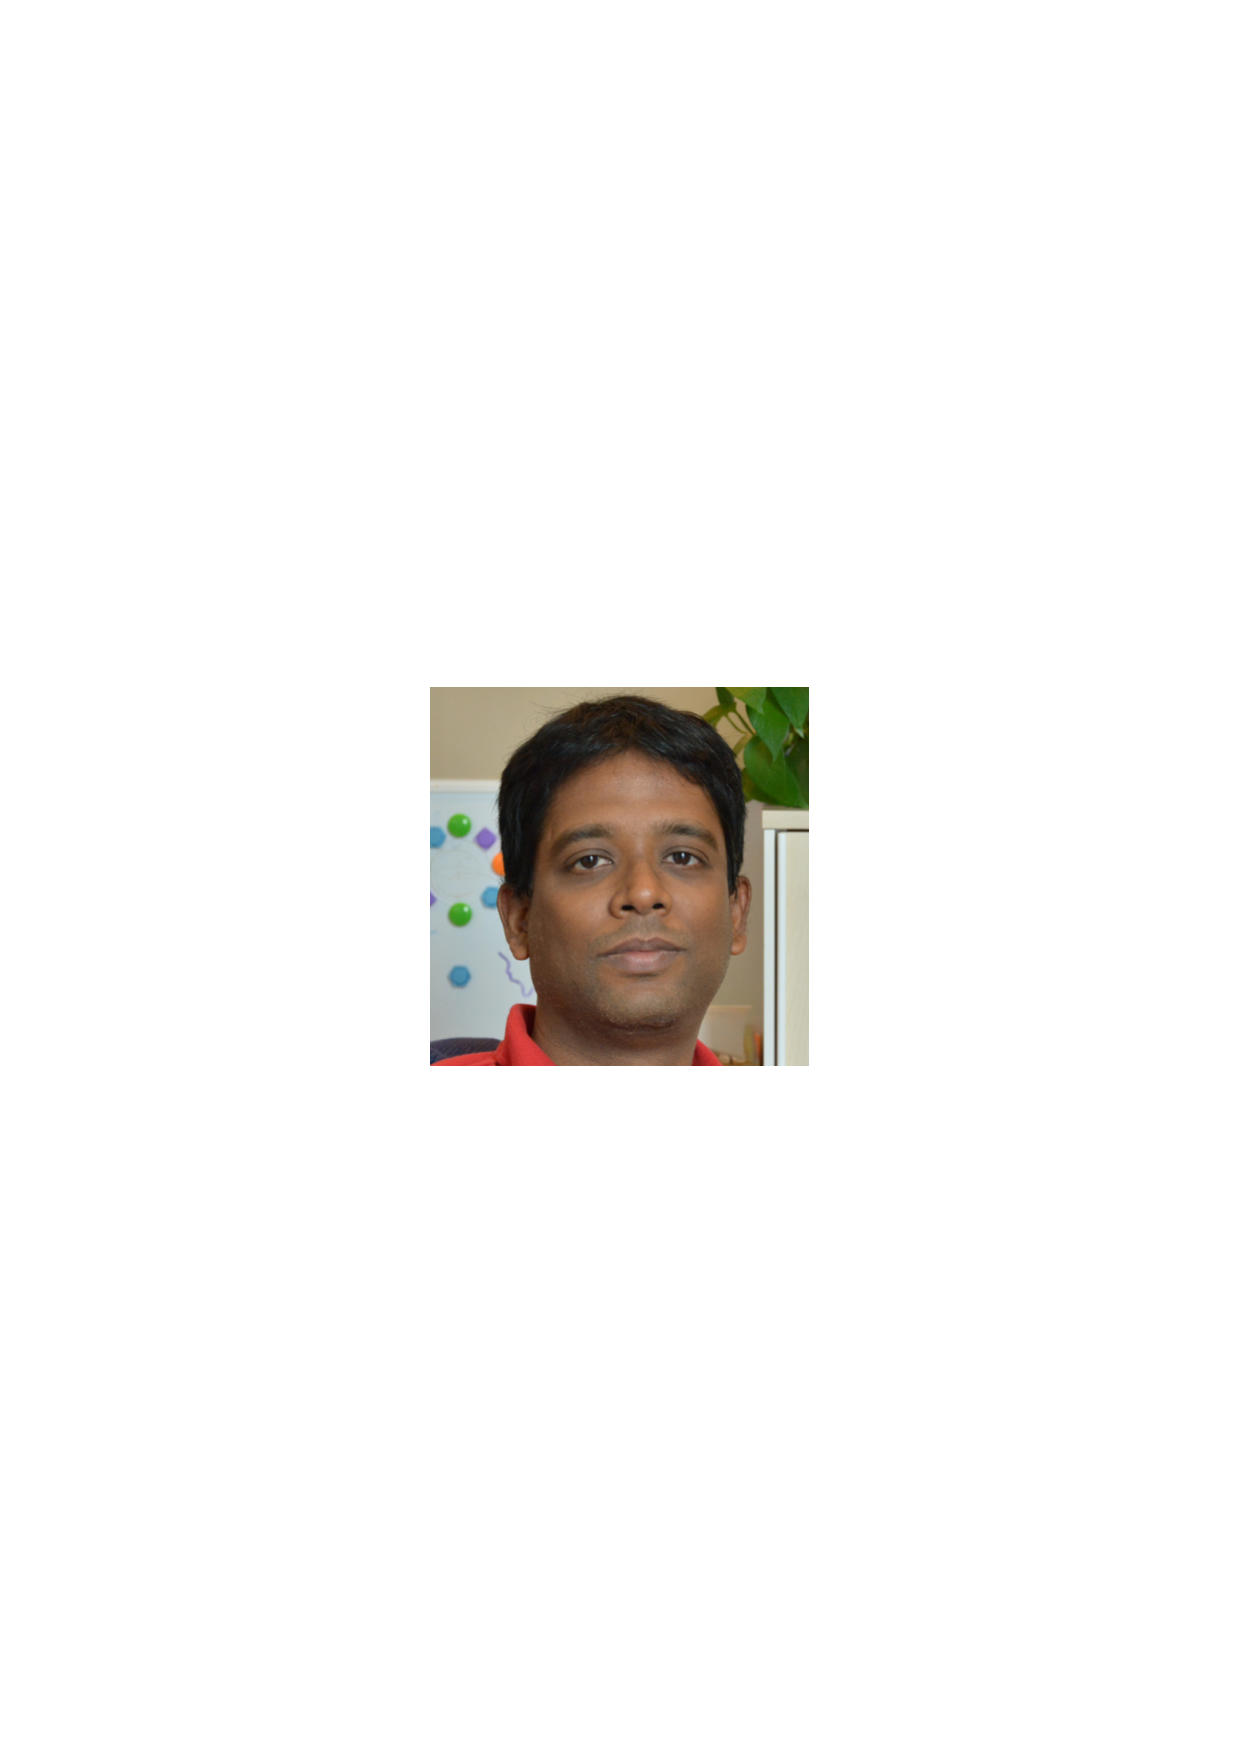
\includegraphics[clip=true, width=0.475\textwidth]{photo_chandra_radhakrishnan}
\end{center}

\dropcap{C}{handrashekar Radhakrishnan} is a Postdoctoral Fellow and Bright Overseas Global Corporation Scholar at New York University, Shanghai, China. He is a recipient of the National Natural Science Foundation of China, International Young Scientist research grant. Before Joining NYU Shanghai he worked as a Postdoctoral Fellow at the Institute of Mathematical Science, India and the National Chung Hsing University, Taiwan. He obtained his Master of Science in Physics from the Indian Institute of Technology Madras and a PhD in theoretical physics from University of Madras. He has worked on a variety of fields, including statistical mechanics, mathematical physics and quantum information theory. His fundamental interest in quantum information theory lies in investigating quantum resources alternative to entanglement, which can be used for quantum communication and quantum computation. He has active collaborations with experimentalists, through which he tries to verify his theoretical results. He also has some interest in the application of statistical mechanics to biological problems.

%
% Jon Dowling
%

\begin{center}
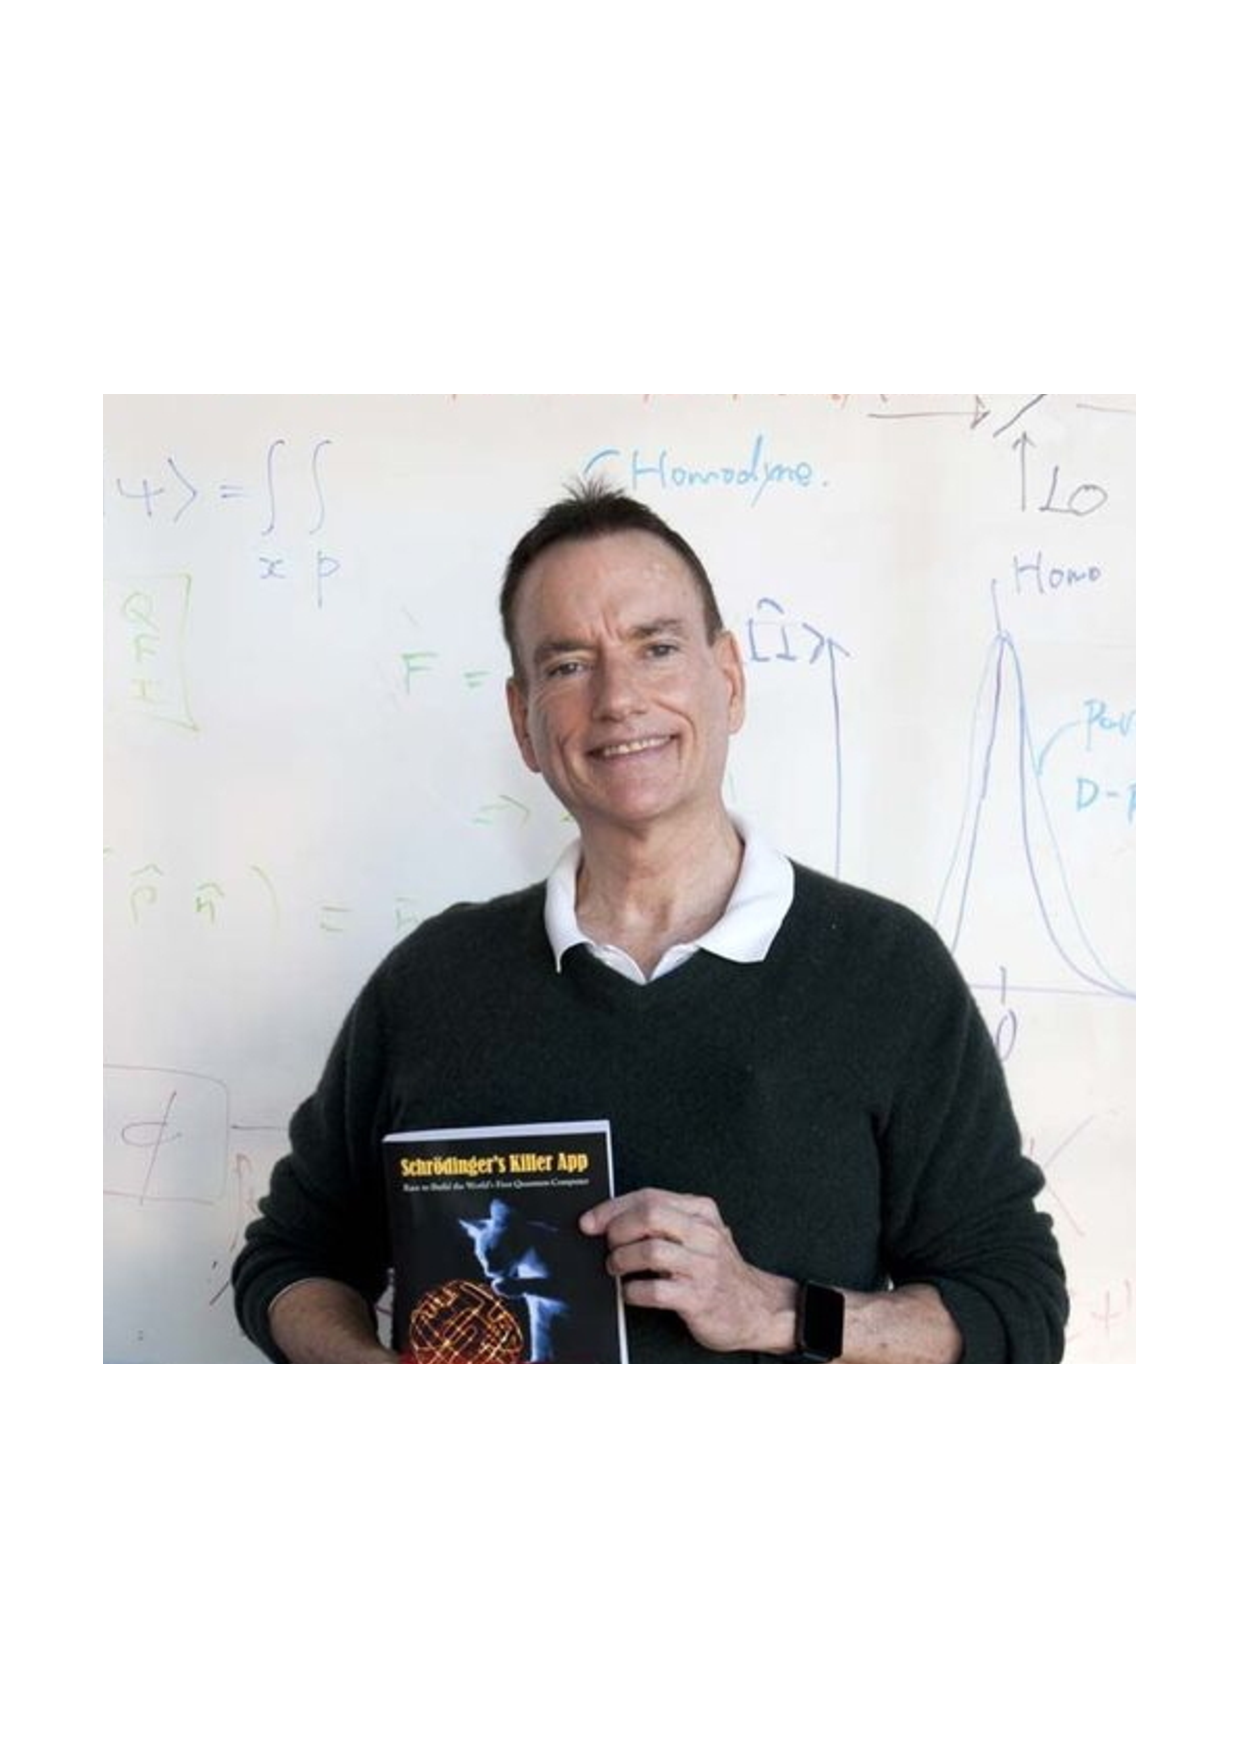
\includegraphics[clip=true, width=0.475\textwidth]{photo_jon_dowling}
\end{center}

\dropcap{J}{on Dowling} is Professor and Hearne Chair of Theoretical Physics, and Co-Director of the Hearne Institute for Theoretical Physics at Louisiana State University. He has a highly-acclaimed research career, with over 450 publications and 15,000 citations. He is author of the popular book \textit{Schr\"odinger's Killer App: Race to Build the World's First Quantum Computer}.

\comment{Complete this section}

%
% Tim Byrnes
%

\begin{center}
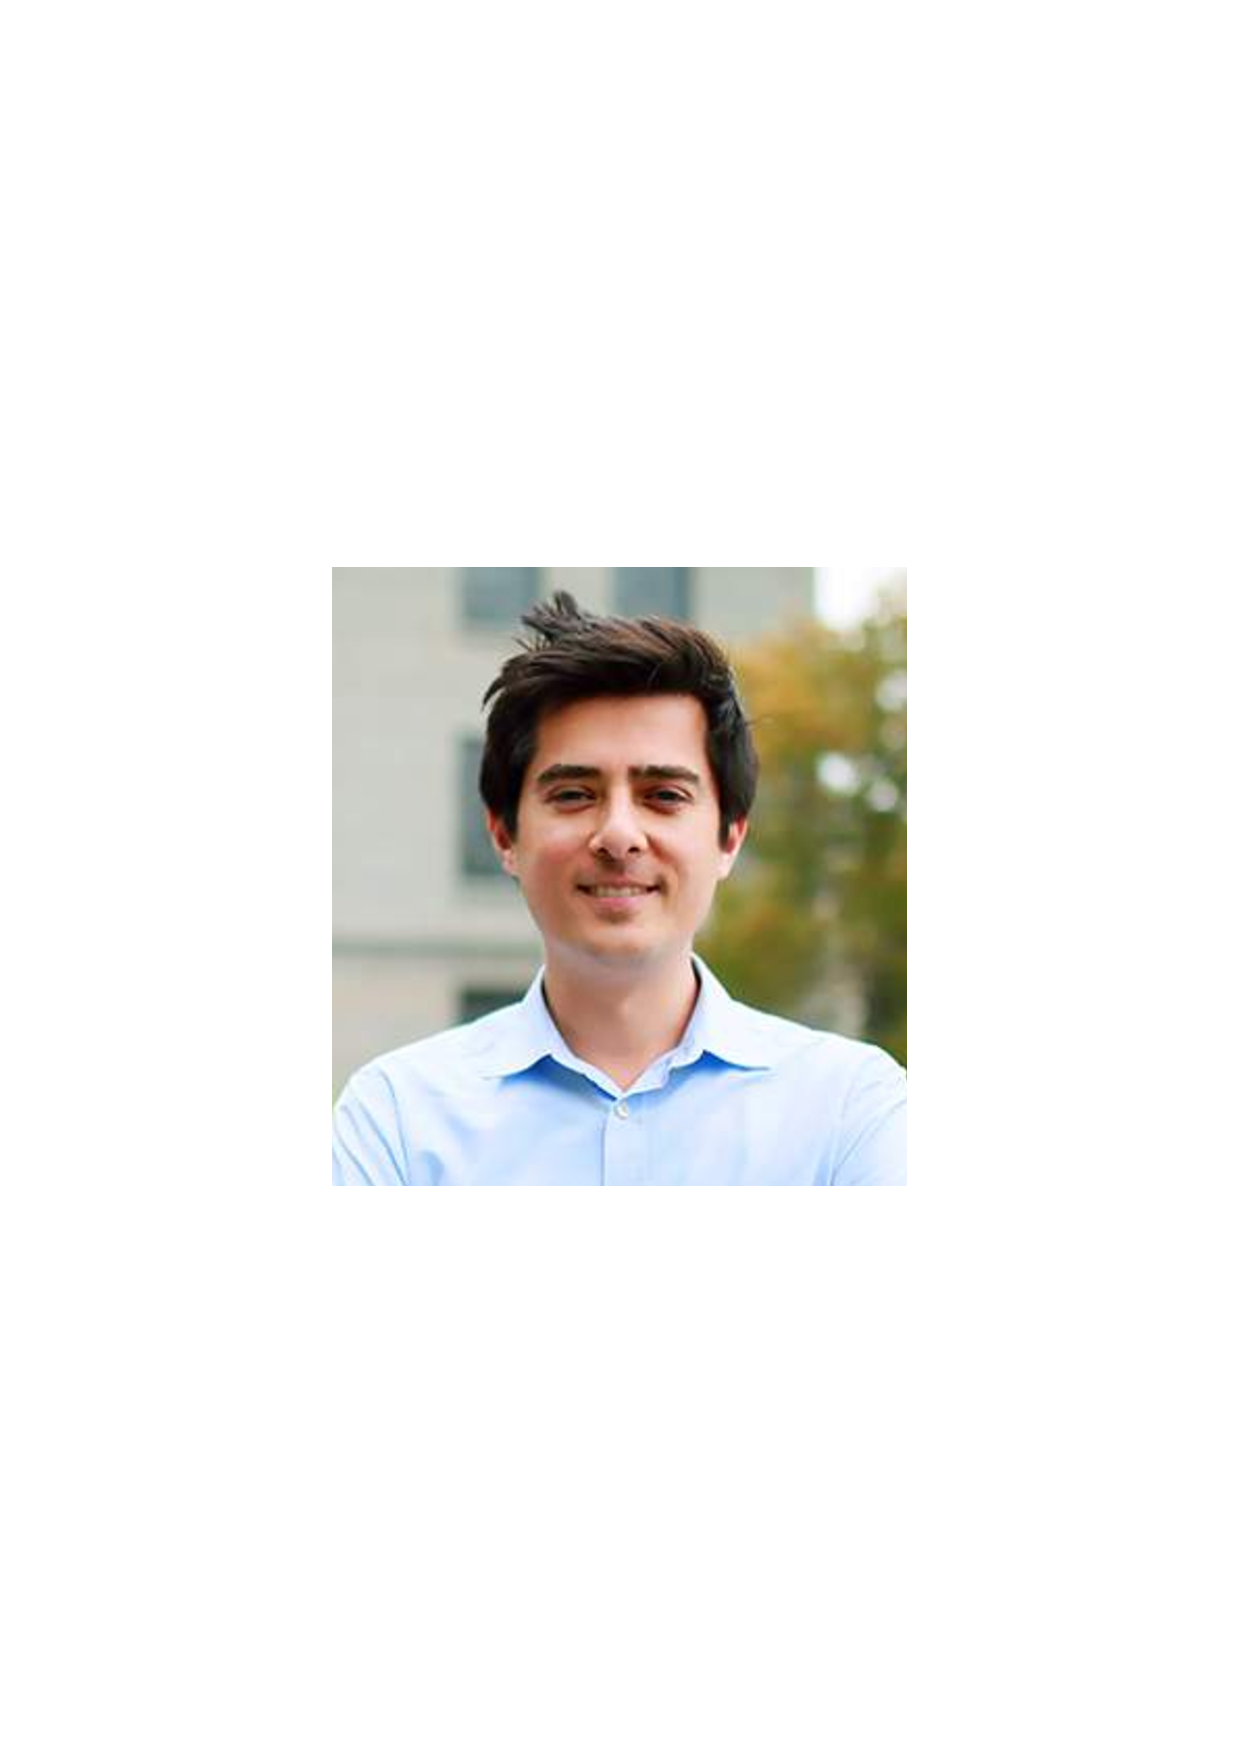
\includegraphics[clip=true, width=0.475\textwidth]{photo_tim_byrnes}
\end{center}

\dropcap{T}{im Byrnes}....

\comment{Complete this section}

%
% Bill Munro
%

\begin{center}
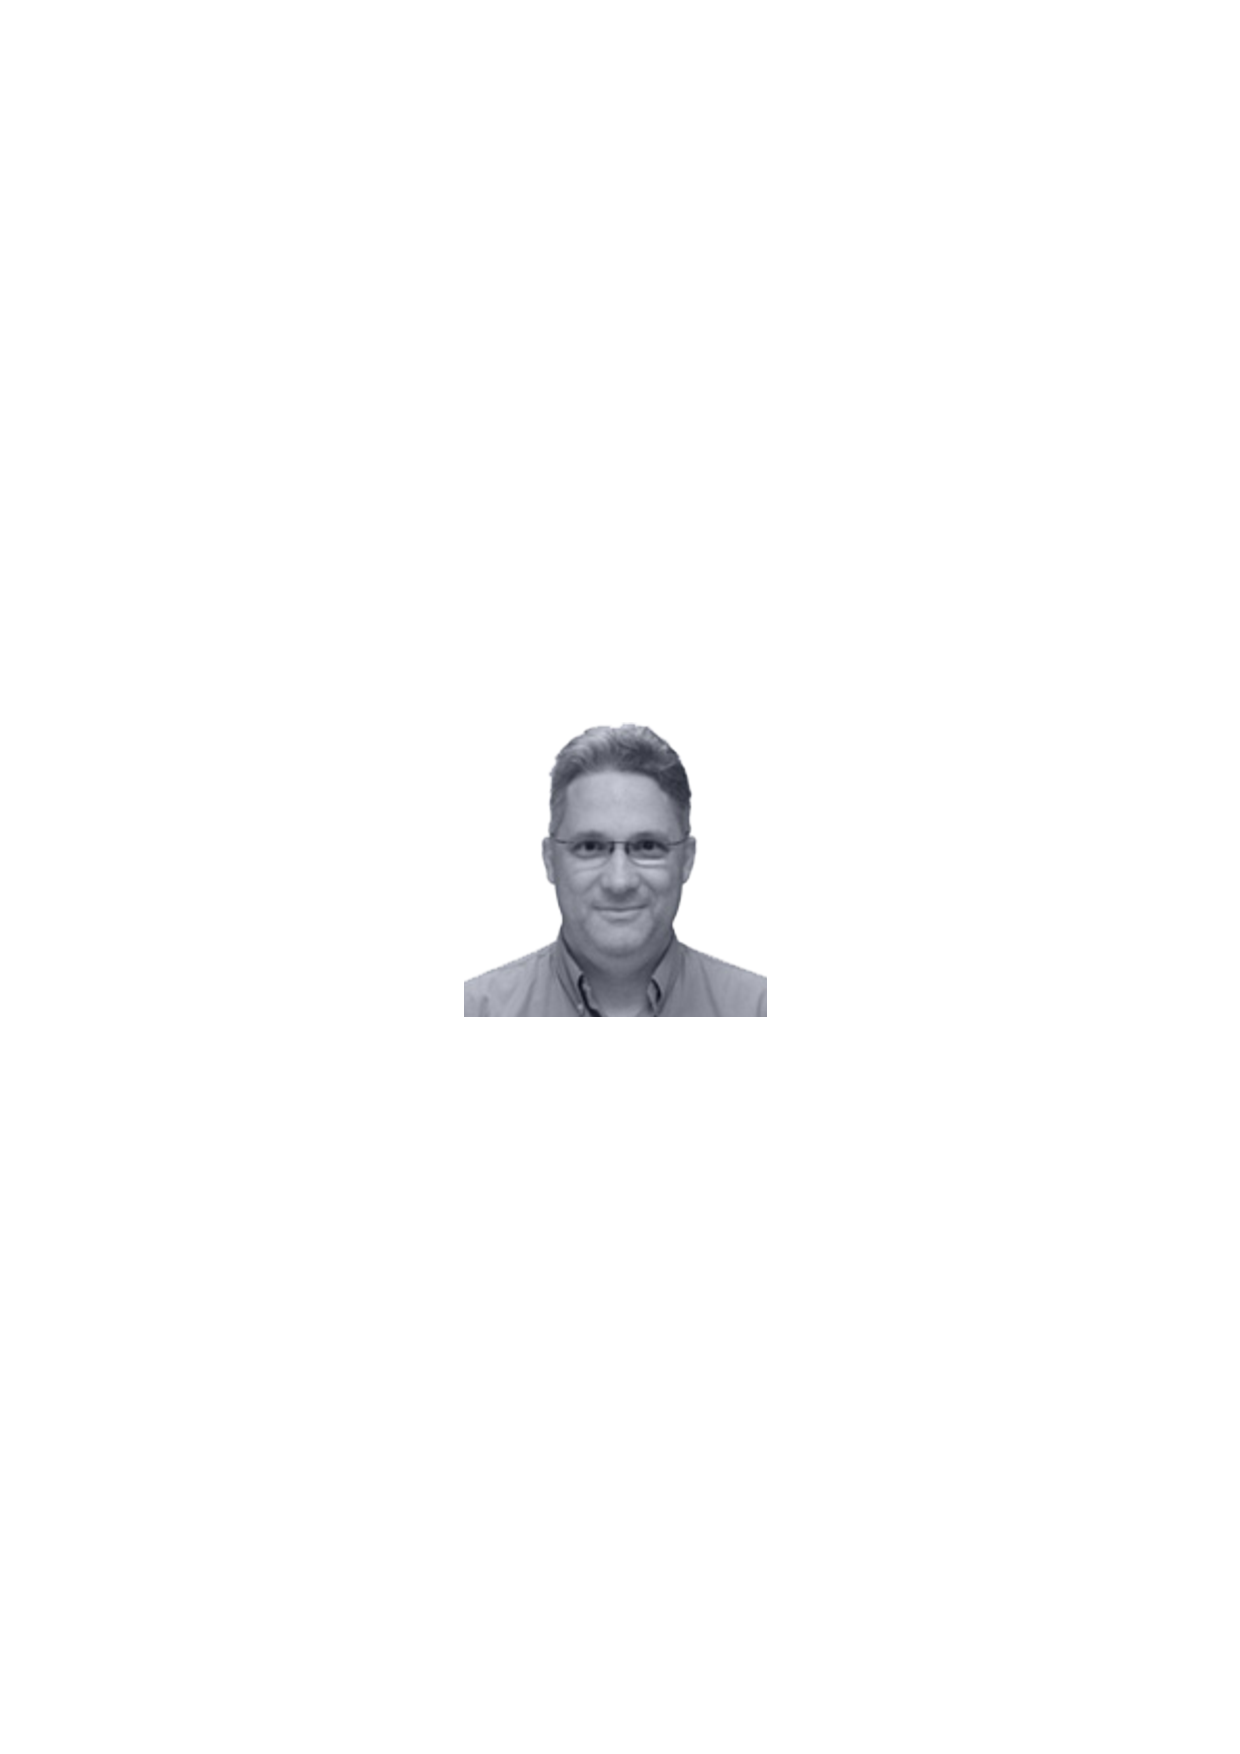
\includegraphics[clip=true, width=0.475\textwidth]{photo_bill_munro}
\end{center}

\dropcap{B}{ill Munro} obtained his PhD at the University of Waikato, and has since held numerous prestigious fellowships and positions. He is currently Senior Research Scientist and leader of the theoretical quantum physics research group at NTT Japan.

\comment{Complete this section}